\section{答案与解析：结构力学基础与技巧班第3次作业答案（材料力学回顾）}
\begin{analysisbox}
弯矩图、剪力图和轴力图要先确定支座反力，再按截面法分段。符号约定要前后一致，最大应力或变形应结合截面几何量与材料参数检查量纲。
\end{analysisbox}
\subsection*{第 1 页转写}
一、

（a）解：取整体隔离体竖向力平衡，可得B处竖向支反力



0

0

1

1

2

2

By

F

l

q

q l

=

\textbackslash{}times \textbackslash{}times

=



对B点取矩得B处支座反力矩

2

0

0

1

1

1

2

3

6

B

M

l

q

l

q l

=-

\textbackslash{}times \textbackslash{}times

\textbackslash{}times

=-

（上侧受拉）

画出原结构弯矩图和剪力图如图（a）（b）所示。

（b ）解：取整体隔离体竖向力平衡，可得A 处竖向支反力

15 1 30

Ay

F

=

\textbackslash{}times +

=



45KN 

，对A 点取矩得A 处支座反力矩

15 1 2.5

30 3

A

M

=-

\textbackslash{}times \textbackslash{}times

-

\textbackslash{}times =

127.5KN m

-



（上侧受拉）。弯矩图如图（a）所示。

（c）解：取整体隔离体对C点取矩，由

3 30 40 1.5 0

B

F \textbackslash{}times +

-

\textbackslash{}times

=

，可得B点竖向支

反力

10

B

F

KN

=

，竖向力平衡得

30

C

F

KN

=

。画出弯矩图如图（b）（c）所示。
\begin{figure}[H]\centering
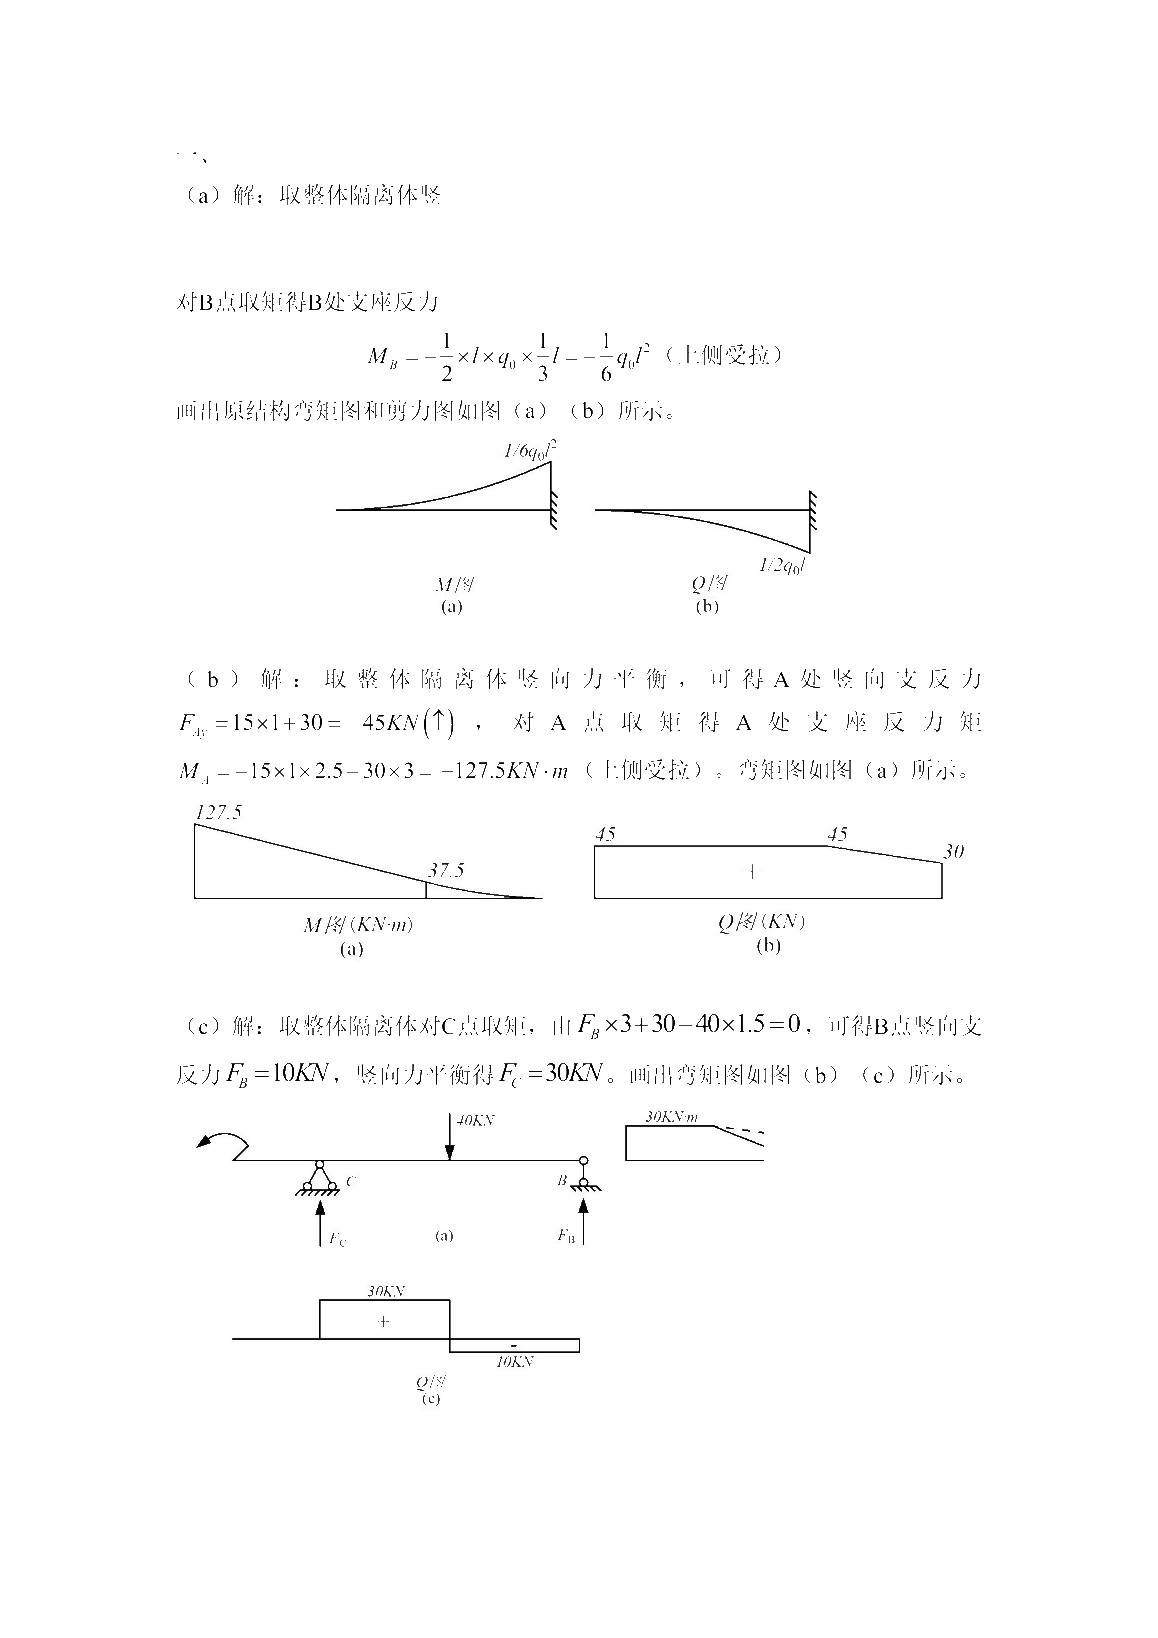
\includegraphics[width=0.92\textwidth]{figures/src05_p001.jpg}
\caption{结构力学基础与技巧班第3次作业答案（材料力学回顾） 第 1 页清理图形页}
\end{figure}
\subsection*{第 2 页转写}
（d）解：取整体隔离体对A点取矩，由

10 4 0.2 10 5 0

B

F \textbackslash{}times

--

\textbackslash{}times

\textbackslash{}times =，可得B点竖向

支反力

1.4

B

F

KN

=

，竖向力平衡得

0.6

A

F

KN

=

。C处作用了集中力偶，两侧截面

的弯矩有突变，由C左侧截开取AC隔离体，可得

0.6 8 0.2 8 4

L

C

M =

\textbackslash{}times -

\textbackslash{}times \textbackslash{}times =1.6KN m

-



（上侧受拉），由C结点力矩平衡得

2.4

R

C

M

KN m

=



（下侧受拉）。画出弯矩图和剪力图如图（b）（c）所示。

（e）解：取整体隔离体对A点取矩，由

3 6 20 2 20

0

B

F \textbackslash{}times --

\textbackslash{}times -

=

，可得B点竖向

支反力

22

B

F

KN

=

，竖向力平衡得

2

A

F

KN

=

。画出弯矩图和剪力图如图（b）（c）

所示。
\begin{figure}[H]\centering
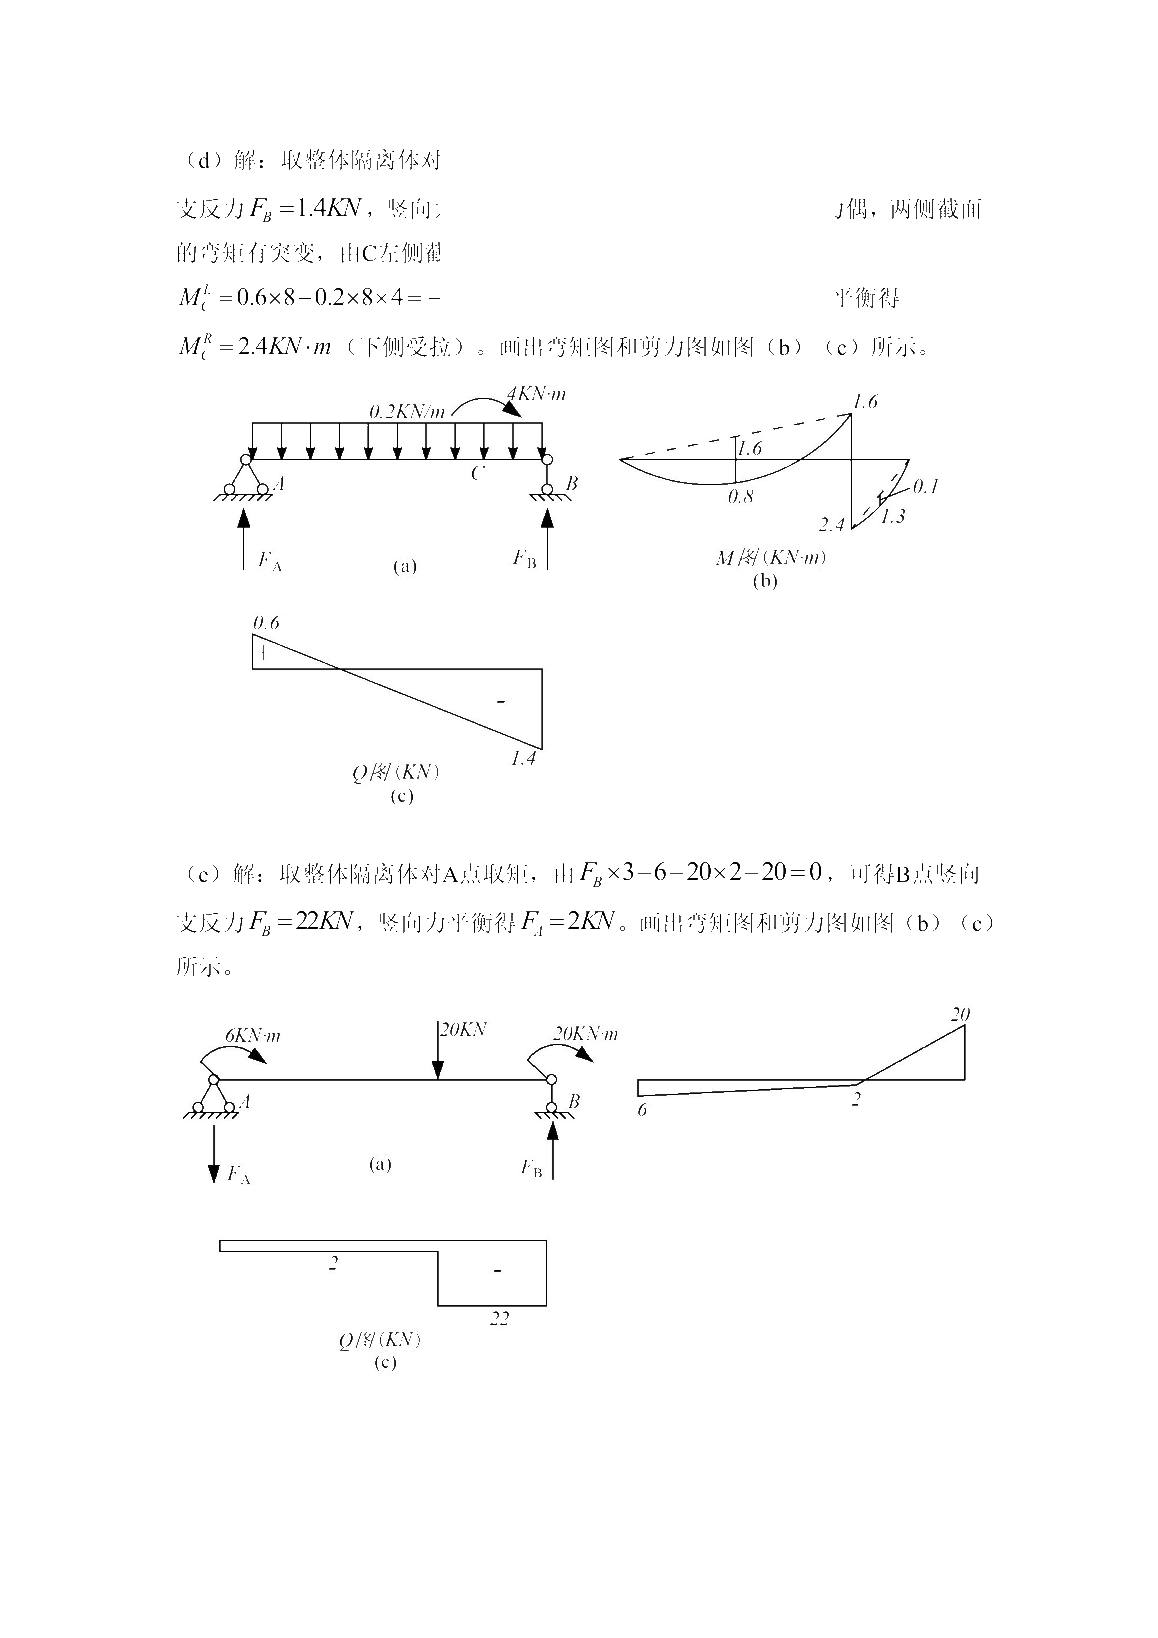
\includegraphics[width=0.92\textwidth]{figures/src05_p002.jpg}
\caption{结构力学基础与技巧班第3次作业答案（材料力学回顾） 第 2 页清理图形页}
\end{figure}
\subsection*{第 3 页转写}
（f）解：取整体隔离体对A点取矩，由

4

4.5

0

C

F

a q a

a

\textbackslash{}times

-\textbackslash{}times \textbackslash{}times

=，可得B点竖向支

反力

1.125

C

F

qa

=

，竖向力平衡得

0.125

A

F

qa

=

。画出弯矩图和剪力图如图（b）

（c）所示。

二、

（a）解：取整体隔离体竖向力平衡，可得A处竖向支反力



5 1

5

Ay

F

KN

=

\textbackslash{}times =



对A点取矩得A处支座反力矩

5 1 2

10

A

M

KN m

=-\textbackslash{}times \textbackslash{}times =-



（上侧受拉）

画出弯矩图和剪力图如图（a）（b）所示。

（b）解：取整体隔离体竖向力平衡，可得A处竖向支反力



15

Ay

F

KN

=



对A点取矩得A处支座反力矩

10 15 1

25

A

M

KN m

=-

-

\textbackslash{}times =-



（上侧受拉）

画出弯矩图和剪力图如图（a）（b）所示。
\begin{figure}[H]\centering
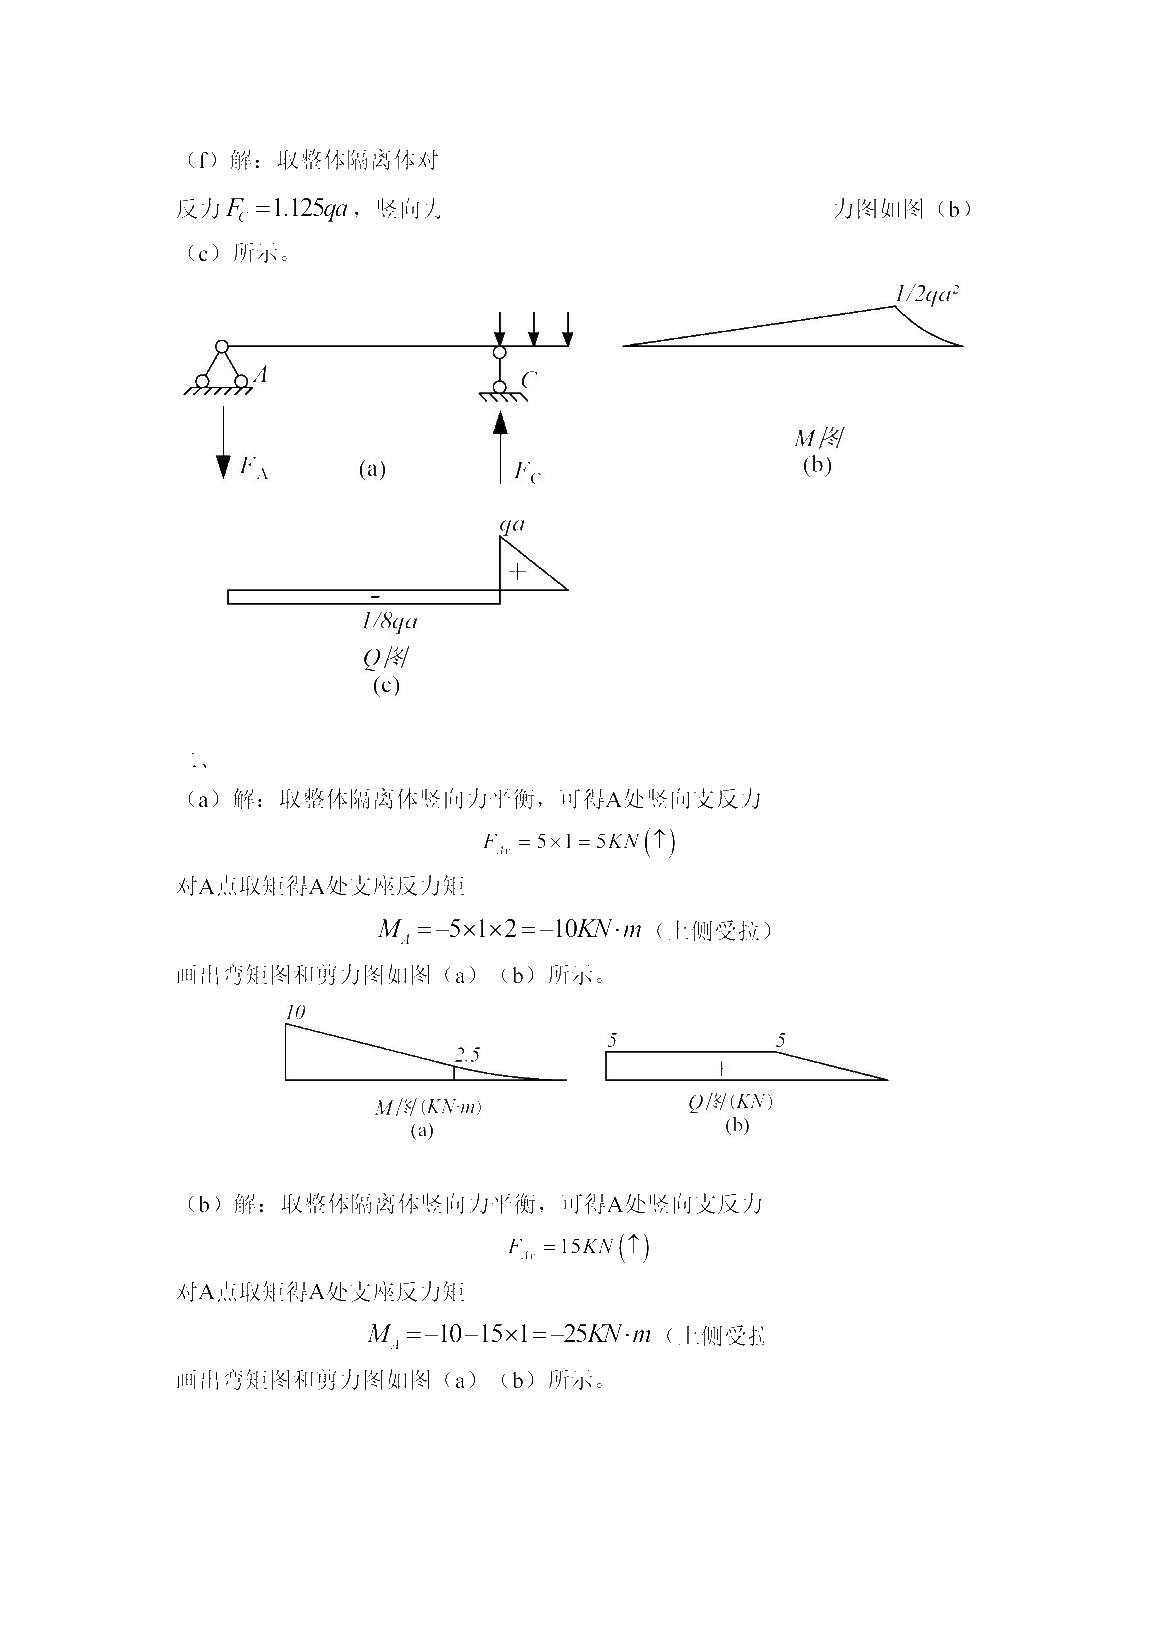
\includegraphics[width=0.92\textwidth]{figures/src05_p003.jpg}
\caption{结构力学基础与技巧班第3次作业答案（材料力学回顾） 第 3 页清理图形页}
\end{figure}
\subsection*{第 4 页转写}
（c）解：取整体隔离体对A点取矩，由

5

3

2.5

0

B

F

a q

a

a

\textbackslash{}times

-\textbackslash{}times

\textbackslash{}times

=，可得B点竖向

支反力

1.5

B

F

qa

=

，竖向力平衡得

1.5

A

F

qa

=

。画出弯矩图和剪力图如图（b）（

c）所示。

（d）解：取整体隔离体对A点取矩，由

3

2

0

B

e

e

F

a M

M

\textbackslash{}times

+

-

=

，可得B点竖向支

反力

3

e

B

M

F

a

=

，竖向力平衡得

3

e

A

M

F

a

=

。画出弯矩图和剪力图如图（b）（c）所

示。
\begin{figure}[H]\centering
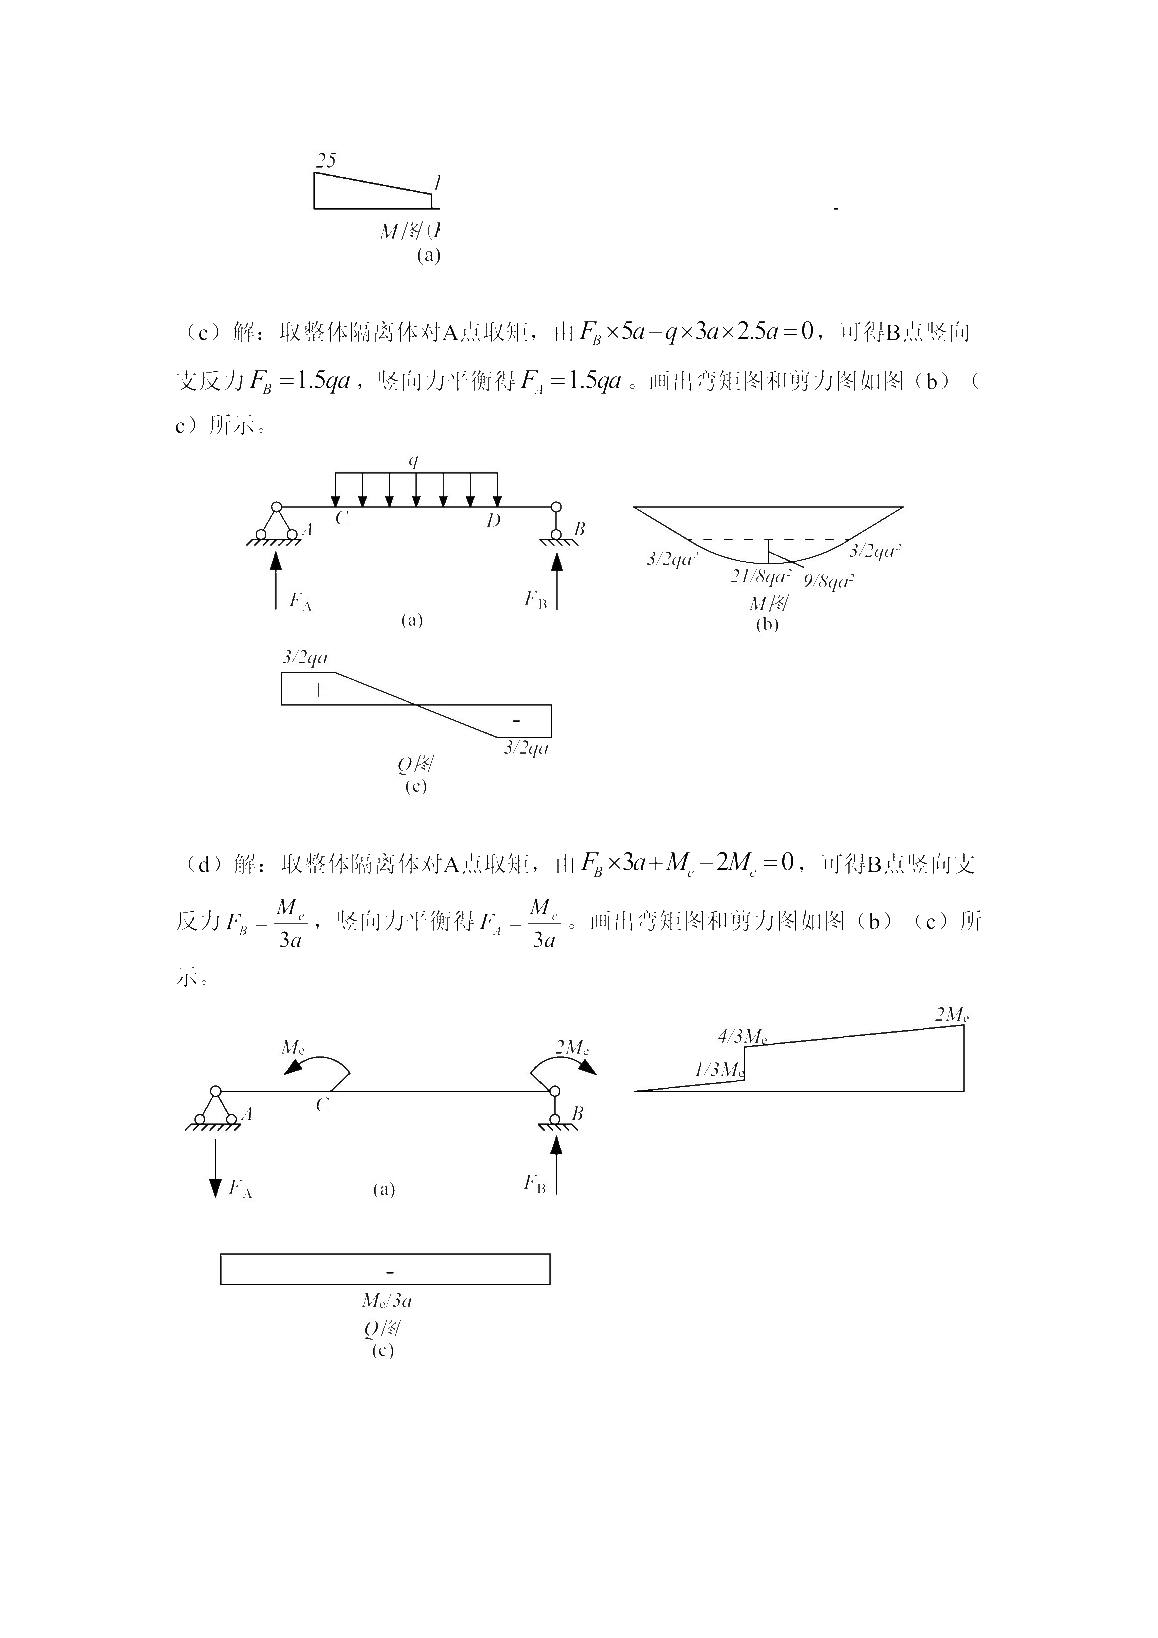
\includegraphics[width=0.92\textwidth]{figures/src05_p004.jpg}
\caption{结构力学基础与技巧班第3次作业答案（材料力学回顾） 第 4 页清理图形页}
\end{figure}
\subsection*{第 5 页转写}
（e）解：取整体隔离体对A点取矩，由

4 4 4 2 4 20

B

F \textbackslash{}times =\textbackslash{}times \textbackslash{}times ++

可得B处支座反力

14

B

F

KN

=

。再由整体竖向力平衡，可得A处支座反力

2

A

F

KN

=

。画出弯矩图和

剪力图如图（b）（c）所示。

（f）解：取整体隔离体对A点取矩，由

11

4

2

3

8

B

F

a

F

a

F

a

F

a

\textbackslash{}times

+

\textbackslash{}times

=

\textbackslash{}times

+

\textbackslash{}times

，可得B

处支座反力

5

16

B

F

F

=

，再由整体竖向力平衡，可得A处支座反力

5

16

A

F

F

=

。画

出弯矩图和剪力图如图（b）（c）所示。
\begin{figure}[H]\centering
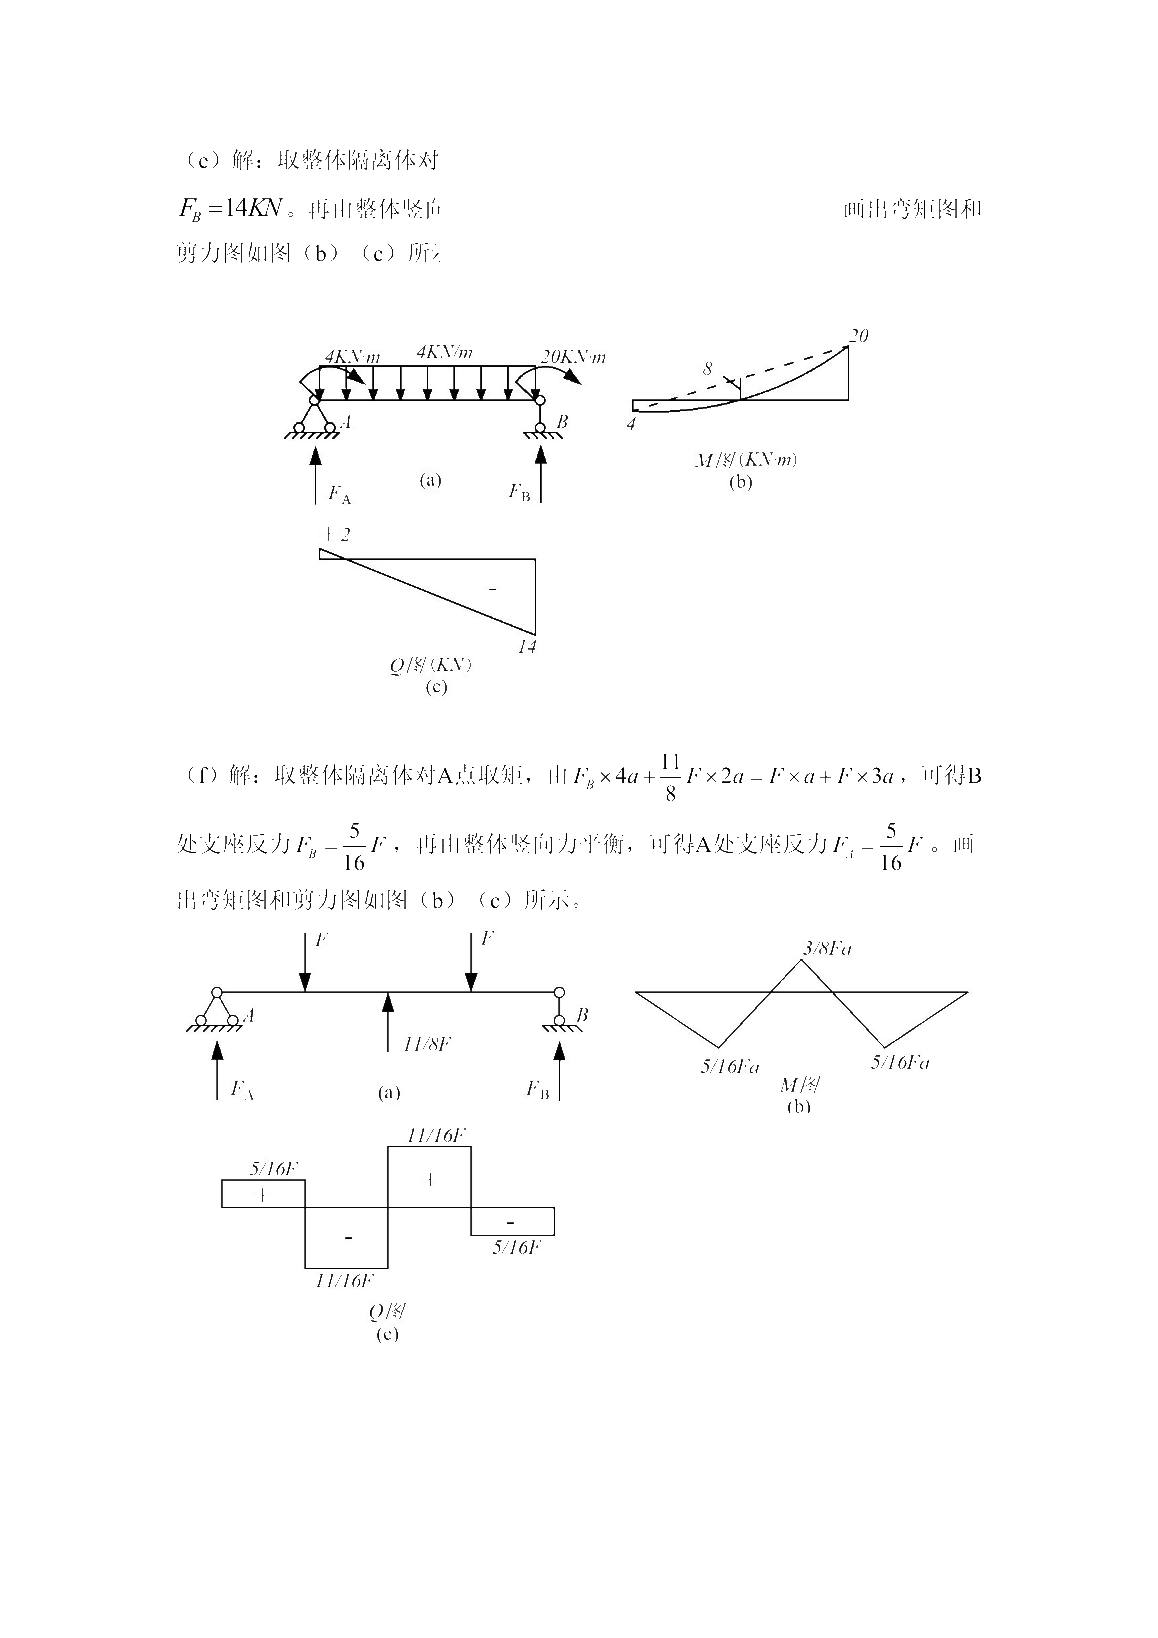
\includegraphics[width=0.92\textwidth]{figures/src05_p005.jpg}
\caption{结构力学基础与技巧班第3次作业答案（材料力学回顾） 第 5 页清理图形页}
\end{figure}
\subsection*{第 6 页转写}
（g）解：取整体隔离体对A点取矩，由

2

2 1 0.5

B

F \textbackslash{}times =\textbackslash{}times \textbackslash{}times

可得B结点的竖向反力

1

2

B

F

KN

=

，再由整体竖向力平衡，可得A处支座反力

3

2

A

F =

。画出弯矩图和剪

力图如图（b）（c）所示。

（h）解：取整体隔离体对A点取矩，由

6 10 6 3 250 2 250 4

B

F \textbackslash{}times =

\textbackslash{}times \textbackslash{}times +

\textbackslash{}times +

\textbackslash{}times 可得B

处支座的竖向反力

280

B

F

KN

=

，再由整体竖向力平衡，可得A处支座反力

280

A

F

KN

=

。画出弯矩图和剪力图如图（b）（c）所示。

三、
\begin{figure}[H]\centering
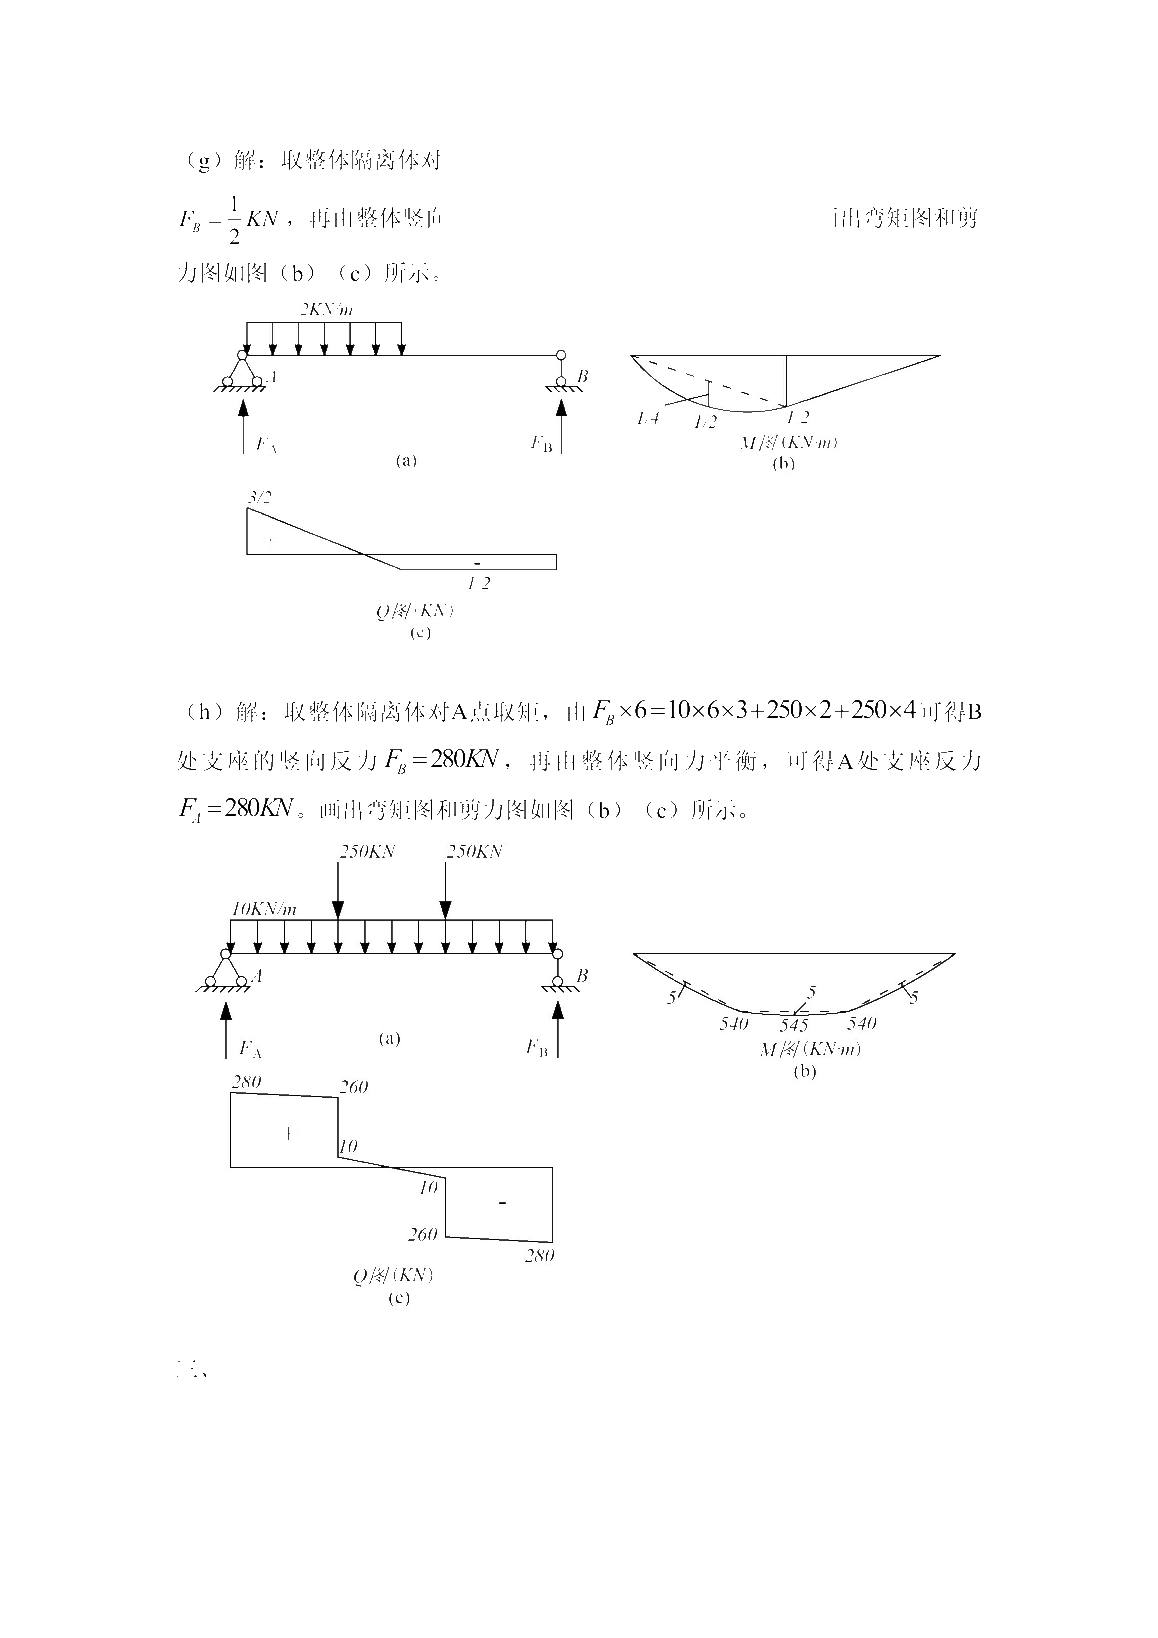
\includegraphics[width=0.92\textwidth]{figures/src05_p006.jpg}
\caption{结构力学基础与技巧班第3次作业答案（材料力学回顾） 第 6 页清理图形页}
\end{figure}
\subsection*{第 7 页转写}
（a）解：取CD部分隔离体并对B点取矩，由

C

F

a

qa a

\textbackslash{}times =

\textbackslash{}times 可得C结点的竖向反

力

C

F

qa

=

，再取AC部分，可得A处固定端反力矩

2

2

1

1

2

2

A

M

qa a

qa

qa

=

\textbackslash{}times

-

=

（下

侧受拉）。画出弯矩图和剪力图如图（b）（c）所示。

（b）解：已知AC为二力杆，没有剪力和弯矩，易画出弯矩图和剪力图如图（a）

（b）所示。
\begin{figure}[H]\centering
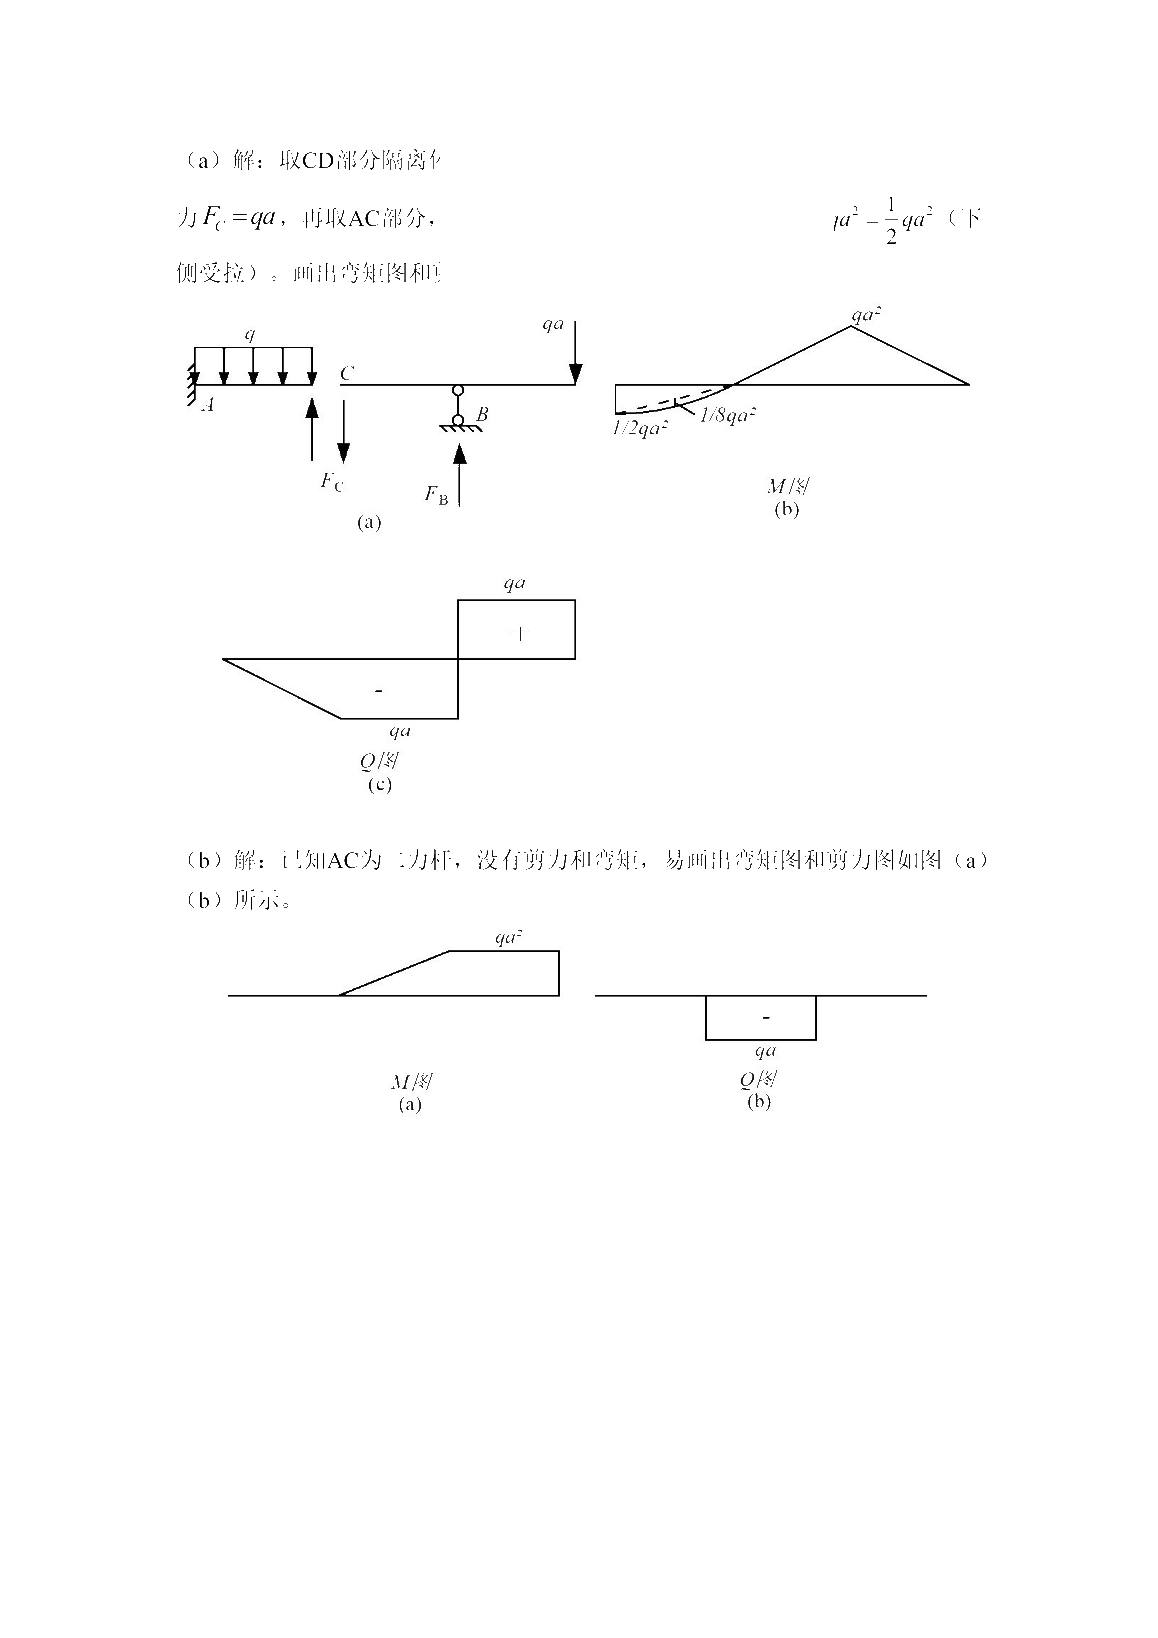
\includegraphics[width=0.92\textwidth]{figures/src05_p007.jpg}
\caption{结构力学基础与技巧班第3次作业答案（材料力学回顾） 第 7 页清理图形页}
\end{figure}
